%=========== ΛΥΣΗ - 67ο ΘΕΜΑ Δ ===========
\begin{thema}{Δ}
\begin{erwthma}
\item Από το σχήμα της $C_{f'}$ έχουμε
\[
f'(x)>0,\quad x\in(0,4),
\]
και
\[
f'(x)<0,\quad x\in(4,8).
\]
Άρα η $f$ είναι \textbf{γνησίως αύξουσα} στο $[0,4]$ και
\textbf{γνησίως φθίνουσα} στο $[4,8]$.

Ο πίνακας μεταβολών της $f$ είναι:
\begin{center}
\begin{tikzpicture}
\tkzTabInit[color,lgt=2.2,espcl=1.8,
colorC=maincolor!50!white,colorL=maincolor!20!white,
colorV=maincolor!50!white]%
{$x$/.8,$f'(x)$/.8,$f(x)$/1.2}%
{$0$,$4$,$8$}%
\tkzTabLine{z,+,z,-,z}
\tkzTabVar{-/{$f(0)=0$},+/{$f(4)$},-/{$f(8)$}}
\end{tikzpicture}
\end{center}

Επομένως η $f$ παρουσιάζει ολικό μέγιστο στο $x=4$, με τιμή $f(4)$.
Επιπλέον, επειδή $f(0)=0$, έχουμε
\[
f(8)-f(0)=\int_0^8 f'(x)\d x.
\]
Το ολοκλήρωμα αυτό είναι προσημασμένο εμβαδόν:
\[
\int_0^8 f'(x)\d x=E_+-E_-.
\]
Αφού από τη συμμετρία δίνεται ότι
\[
E_+=E_-,
\]
προκύπτει
\[
\int_0^8 f'(x)\d x=0.
\]
Άρα
\[
f(8)-f(0)=0.
\]
Επειδή $f(0)=0$, καταλήγουμε ότι
\[
{f(8)=0}.
\]
Συνεπώς η $f$ έχει ολικό ελάχιστο στα άκρα $x=0$ και $x=8$, με τιμή
\[
{\min_{[0,8]}f=0}.
\]

\item Η $f$ είναι συνεχής στο $[0,8]$ και παραγωγίσιμη στο $(0,8)$.
Επιπλέον, από το προηγούμενο ερώτημα έχουμε
\[
f(0)=f(8)=0.
\]
Άρα εφαρμόζεται το θεώρημα \eng{Rolle} στο $[0,8]$, οπότε υπάρχει
$\xi\in(0,8)$ τέτοιο ώστε
\[
f'(\xi)=0.
\]
Από το σχήμα γνωρίζουμε ότι η $f'$ μηδενίζεται μόνο στα
\[
x=0,\quad x=4,\quad x=8.
\]
Άρα η μοναδική ρίζα της $f'$ στο $(0,8)$ είναι
\[
{\xi=4}.
\]

Τώρα εφαρμόζουμε το θεώρημα \eng{Rolle} στη συνάρτηση $f'$.

Στο διάστημα $[0,4]$ η $f'$ είναι συνεχής και παραγωγίσιμη στο $(0,4)$,
αφού η $f$ είναι δύο φορές παραγωγίσιμη. Επίσης
\[
f'(0)=f'(4)=0.
\]
Άρα υπάρχει
\[
x_1\in(0,4)
\]
τέτοιο ώστε
\[
(f')'(x_1)=0\Leftrightarrow f''(x_1)=0.
\]

Ομοίως, στο διάστημα $[4,8]$ έχουμε
\[
f'(4)=f'(8)=0,
\]
οπότε, εφαρμόζοντας ξανά το θεώρημα \eng{Rolle} στη $f'$, υπάρχει
\[
x_2\in(4,8)
\]
τέτοιο ώστε
\[
f''(x_2)=0.
\]

Επομένως η εξίσωση $f''(x)=0$ έχει τουλάχιστον δύο ρίζες στο $(0,8)$,
μία στο $(0,4)$ και μία στο $(4,8)$.

\item Έστω
\[
c\in(0,f(4)).
\]
Στο διάστημα $[0,4]$ η $f$ είναι συνεχής και γνησίως αύξουσα, με
\[
f(0)=0<c<f(4).
\]
Άρα, από το θεώρημα \eng{Bolzano}, υπάρχει μία ρίζα
\[
\rho_1\in(0,4)
\]
της εξίσωσης $f(x)=c$. Επειδή η $f$ είναι γνησίως αύξουσα στο $[0,4]$,
η ρίζα αυτή είναι μοναδική στο $(0,4)$.

Στο διάστημα $[4,8]$ η $f$ είναι συνεχής και γνησίως φθίνουσα, με
\[
f(4)>c>0=f(8).
\]
Άρα υπάρχει μία ρίζα
\[
\rho_2\in(4,8)
\]
της εξίσωσης $f(x)=c$. Επειδή η $f$ είναι γνησίως φθίνουσα στο $[4,8]$,
η ρίζα αυτή είναι μοναδική στο $(4,8)$.

Συνεπώς, για κάθε $c\in(0,f(4))$, η εξίσωση $f(x)=c$ έχει στο $(0,8)$
\[
{\text{ακριβώς δύο λύσεις}}.
\]

\item Το υλικό σημείο έχει τεταγμένη
\[
y(t)=f(x(t)).
\]
Παραγωγίζοντας ως προς τον χρόνο $t$, παίρνουμε
\[
y'(t)=f'(x(t))\cdot x'(t).
\]
Τη χρονική στιγμή $t_0$ είναι $x(t_0)=2$ και δίνεται ότι
\[
x'(t_0)=1.
\]
Από το σχήμα διαβάζουμε ότι το σημείο $(2,3)$ είναι σημείο της $C_{f'}$,
δηλαδή
\[
f'(2)=3.
\]
Άρα
\[
y'(t_0)=f'(2)\cdot x'(t_0)=3\cdot1=3.
\]
Επομένως ο ρυθμός μεταβολής της τεταγμένης είναι
\[
{y'(t_0)=3\ \text{μονάδες/sec}}.
\]

Η εφαπτομένη της $C_f$ στο σημείο με τετμημένη $x=2$ έχει συντελεστή
διεύθυνσης
\[
\lambda=f'(2)=3.
\]
Αν $\omega$ είναι η γωνία που σχηματίζει η εφαπτομένη με τον άξονα
$x'x$, τότε
\[
\tan\omega=\lambda.
\]
Άρα
\[
{\tan\omega=3}.
\]
\end{erwthma}
\end{thema}
%=========== ΤΕΛΟΣ ΛΥΣΗΣ - 67ο ΘΕΜΑ Δ ===========
